\usepackage{amsthm}

\newtheorem{theorem}{Theorem}[chapter]
\newtheorem{lemma}           [theorem] {Lemma}   
\newtheorem{folg}           [theorem] {Folgerung}   

\newtheorem{frage}       [theorem] {Frage}   
\newtheorem{question}       [theorem] {Question}   
\newtheorem{aufgabe}       [theorem] {Aufgabe}   
\newtheorem{exercise}       [theorem] {Exercise}  

\newtheorem{proposition}     [theorem] {Proposition}  
\newtheorem{satz}     [theorem] {Satz}  
\newtheorem{fact}{Fact}
\newtheorem{definition}      [theorem] {Definition} 

\theoremstyle{definition} 
\newtheorem{bemerkung}     [theorem] {Bemerkung}  
\newtheorem{beispiel}       [theorem] {Beispiel}  
\newtheorem{example}       [theorem] {Example}  
\newtheorem*{example*} {Example}  
\newtheorem{notation}       [theorem] {Notation}  
\newtheorem*{Faust}[theorem]{Rule of Thumb}
\newtheorem*{Boxx}[theorem]{Concept}

Now we will define the integral for bounded functions:

\begin{Definition}{}
Let $f:[a,b]\to\mathbb{R}$ be bounded. Then we define the \emph{Riemann upper integral}
\[\overline{\int_a^b}f(x)\, dx:=\inf\left\{\int_a^b\phi(x)\, dx\;:\;\phi\in\mathcal{T}([a,b])\text{ with }\phi\geq f\right\}\]
and the \emph{Riemann lower integral} by
\[\underline{\int_a^b}f(x)\, dx:=\sup\left\{\int_a^b\phi(x)\, dx\;:\;\phi\in\mathcal{T}([a,b])\text{ with }\phi\leq f\right\}.\]
\end{Definition}

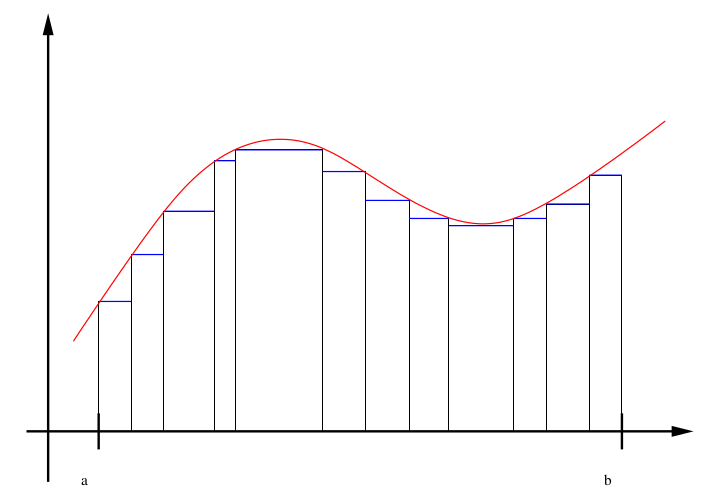
\includegraphics{./lower.png}

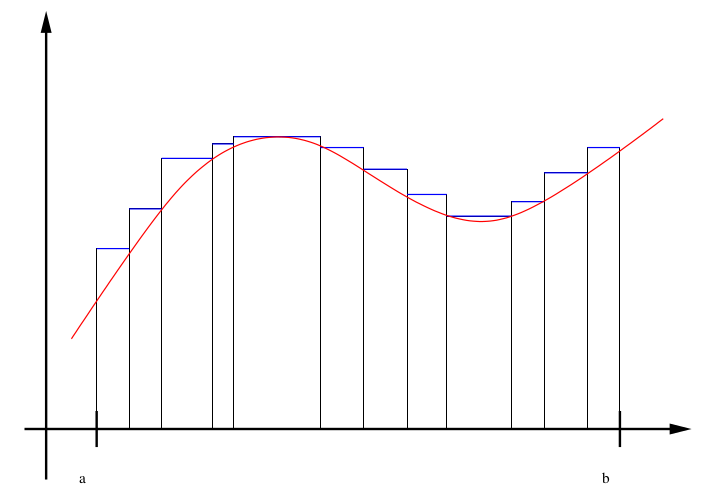
\includegraphics{./upper.png}
% 
It can be seen from the figures above that the integral can be seen as the signed area between the function graph and the $x$-axis. 
\emph{Signed} means that the area of the negative parts of the function has to be counted negative.


By the above definition, we can directly deduce that for $\phi\in\mathcal{T}([a,b])$ holds
\[\overline{\int_a^b}\phi(x)\, dx=\underline{\int_a^b}\phi(x)\, dx={\int_a^b}\phi(x)\, dx.\]

For general bounded functions $f:[a,b]\to\mathbb{R}$ holds
\[\underline{\int_a^b}f(x)\, dx\leq \overline{\int_a^b}f(x)\, dx.\]
Note that in general the upper integral does not coincide with the lower integral. For instance, consider the function $f: [0,1] \to\mathbb{R}$
with
\[f(x)=\begin{cases}1&:\;x\in\mathbb{Q}\\0&:x\in\mathbb{R}\backslash\mathbb{Q}\end{cases}\]
Then we have
\[\overline{\int_0^1}f(x)\, dx=1>0=\underline{\int_0^1}f(x)\, dx.\]
\begin{Theorem}{}
Let $f,g:[a,b]\to\mathbb{R}$ be bounded. Then
\begin{enumerate}[(i)]
\item
\[\overline{\int_a^b}f(x)+g(x)\, dx\leq \overline{\int_a^b}f(x)\, dx+\overline{\int_a^b}g(x)\, dx.\]
\item
\[\underline{\int_a^b}f(x)+g(x)\, dx\geq \underline{\int_a^b}f(x)\, dx+\underline{\int_a^b}g(x)\, dx.\]
\item For $\lambda\geq0$ holds
\[\underline{\int_a^b}\lambda f(x)\, dx=\lambda \underline{\int_a^b}f(x)\, dx,\quad\overline{\int_a^b}\lambda f(x)\, dx=\lambda \overline{\int_a^b}f(x)\, dx.\]
\item For $\lambda\leq0$ holds
\[\underline{\int_a^b}\lambda f(x)\, dx=\lambda \overline{\int_a^b}f(x)\, dx,\quad\overline{\int_a^b}\lambda f(x)\, dx=\lambda \underline{\int_a^b}f(x)\, dx.\]
\end{enumerate}
\end{Theorem}
{\em Proof:}\\
(i) Let $\varepsilon>0$. Then there exist $\phi,\psi\in\mathcal{T}([a,b])$ with $\phi\geq f$, $\psi\geq g$ and
\[
\overline{\int_a^b}f(x)\, dx+\frac\varepsilon2\geq{\int_a^b}\phi(x)\, dx,\qquad
\overline{\int_a^b}g(x)\, dx+\frac\varepsilon2\geq{\int_a^b}\psi(x)\, dx.
\]
Then $f+g\leq\phi+\psi$ and
\[
\begin{aligned}
\overline{\int_a^b}f(x)+g(x)\, dx=&\inf\left\{\int_a^b\zeta(x)\, dx\;:\; \zeta\in\mathcal{T}([a,b])\text{ with }\zeta\geq f+g\right\}\\
\leq& {\int_a^b}\phi(x)+\psi(x)\, dx\\ \leq&
\left(\overline{\int_a^b}f(x)\, dx+\frac\varepsilon2\right)+\left(\overline{\int_a^b}g(x)\, dx+\frac\varepsilon2\right)\\=&
\overline{\int_a^b}f(x)\, dx+\overline{\int_a^b}g(x)\, dx+\varepsilon.
\end{aligned}
\]
Since this holds true for all $\varepsilon>0$, we conclude
\[\overline{\int_a^b}f(x)+g(x)\, dx\leq\overline{\int_a^b}f(x)\, dx+\overline{\int_a^b}g(x)\, dx.\]
(ii): Analogous to (i).\\
(iii):  We only show the statement for the upper integral. The other result can be shown analogously.\\
Let $\varepsilon>0$. Then there exists some $\phi\in\mathcal{T}([a,b])$ with $\phi\geq f$ and
\[\overline{\int_a^b}f(x)\, dx+\varepsilon\geq{\int_a^b}\phi(x)\, dx.\]
Then $\lambda \phi\geq\lambda f$ and
\[\overline{\int_a^b} \lambda f(x)\, dx\leq{\int_a^b}\lambda\phi(x)\, dx=\lambda{\int_a^b}\phi(x)\, dx\leq \lambda\overline{\int_a^b} f(x)\, dx+\lambda\varepsilon.\]
Since this holds true for all $\varepsilon>0$, we conclude
\[\overline{\int_a^b}\lambda f(x)\, dx\leq\lambda \overline{\int_a^b}f(x)\, dx.\]
The opposite inequality follows from the previous one applied to $g(x):=\lambda f(x)$ and $\mu:=\frac{1}{\lambda}>0$:
\[\overline{\int_a^b} f(x)\, dx =  \overline{\int_a^b} \mu g(x)\, dx \leq \mu \overline{\int_a^b}g(x)\, dx = \frac{1}{\lambda} \overline{\int_a^b}\lambda f(x)\, dx.\]
Multiplying this inequality by $\lambda>0$ yields
\[\lambda \overline{\int_a^b} f(x)\, dx  \leq \overline{\int_a^b}\lambda f(x)\, dx.\]

(iv): This result can be shown by using (iii) and the fact
\[\overline{\int_a^b}-f(x)\, dx=-\underline{\int_a^b}f(x)\, dx.\]
\hfill$\Box$

\begin{Definition}{}
A~bounded function $f:[a,b]\to\mathbb{R}$ is called \emph{Riemann-integrable} if
\[\overline{\int_a^b}f(x)\, dx=\underline{\int_a^b}f(x)\, dx.\]
In this case, we write
\[{\int_a^b}f(x)\, dx=\underline{\int_a^b}f(x)\, dx.\]
The set of Riemann-integrable functions is denoted by $\mathcal{R}([a,b])$.
\end{Definition}
%\begin{theorem}
%A~function $f\in\mathcal{B}([a,b])$ is Riemann-integrable if and only if for all $\varepsilon>0$ there exist $\phi,\psi\in\mathcal{T}([a,b])$ %such that $\phi\geq f\geq\psi$ and
%\[\int_a^b\phi(x)-\psi(x)\, dx<\varepsilon.\]
%\end{theorem}


We obviously have that $\mathcal{T}([a,b])\subset\mathcal{R}([a,b])$. In the following we state that monotonic functions as well as continuous functions are Riemann-integrable. The proof is not presented here.

\begin{Remark}{}
As it holds true for summation, the integration variable can be renamed without changing the integral. That is, for $f\in\mathcal{R}([a,b])$ holds
\[{\int_a^b}f(x)\, dx={\int_a^b}f(t)\, dt.\]
\end{Remark}


\begin{Theorem}{}
Let $f:[a,b]\to\mathbb{R}$ be continuous or monotonic. Then $f$ is Riemann-integrable.
\end{Theorem}

The following result is straightforward:

\begin{Theorem}{}
$\mathcal{R}([a,b])$ is a real vector space and the mapping
\[\int_a^b\;:\;\mathcal{R}([a,b])\to\mathbb{R}\]
is linear and monotonic.
\end{Theorem}


